\documentclass[12pt, oneside]{article}
\usepackage[letterpaper, margin=1in, headsep=0.5in]{geometry}
\usepackage[english]{babel}
\usepackage[utf8]{inputenc}
\usepackage{amsmath}
\usepackage{amsfonts}
\usepackage{amssymb}
\usepackage{tikz}
\usetikzlibrary{angles}
\usepackage{graphicx}
%\usepackage{tkz-fct}
%\usepackage{pgfplots}
%\pgfplotsset{width=10cm,compat=1.9}
%\usepgfplotslibrary{statistics}
%\usepackage{pgfplotstable}
%\usepackage{venndiagram}

\usepackage{fancyhdr}
\pagestyle{fancy}
\fancyhf{}
\lhead{BECA / Dr. Huson / Geometry\\* Vocabulary \& notation problem bank}

\renewcommand{\headrulewidth}{0pt}

\begin{document}
\subsection*{Homework 1.1 HW, 1.3 DNQ}

\begin{enumerate}
  \item A(n) $\rule{4cm}{0.15mm}$ is a straight continuous arrangement of an infinite number of points.
  \item A(n) $\rule{4cm}{0.15mm}$ is a portion of a line that begins with a single point and extends infinitely in one direction.
  \item Points that are all located on the same line are $\rule{4cm}{0.15mm}$.
  \item The points where a line segment begins and ends are the $\rule{4cm}{0.15mm}$.
  \item Two or more line segments of equal measure are $\rule{4cm}{0.15mm}$.
  \item A(n) $\rule{4cm}{0.15mm}$ is a portion of a line that includes two points and all of the collinear points between the two points.
  \item A flat surface is a(n) $\rule{4cm}{0.15mm}$.

\subsection*{Constructions}
  \item Use each term according to its geometric meaning: ``sketch", ``draw", ``construct".
  \item $\rule{4cm}{0.15mm}$ is to make a freehand diagram showing important features.
  \item $\rule{4cm}{0.15mm}$ is to depict with accurate measures using ruler, protractor, and compass.
  \item $\rule{4cm}{0.15mm}$ is a formal, logical process to create geometric figures using only a straightedge and compass.

\subsection*{Notation}
  \item Use symbols to write the name of each geometric figure.
  \begin{enumerate}
  \item %Ray DE
    \begin{tikzpicture}
      \draw [->, thick] (0,0)--(3,1.5);
      \draw [fill] (0,0) circle [radius=0.05] node[below]{$D$};
      \draw [fill] (2,1) circle [radius=0.05] node[below]{$E$};
    \end{tikzpicture}
  \item \hspace{1cm}%Line AB
    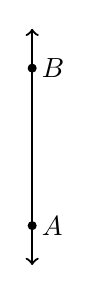
\begin{tikzpicture}
      \draw [<->, thick] (1,0)--(1,3);
      \draw [fill] (1,0.5) circle [radius=0.05] node[right]{$A$};
      \draw [fill] (1,2.5) circle [radius=0.05] node[right]{$B$};
    \end{tikzpicture}
    \item %Line segment XY
      \begin{tikzpicture}
        \draw [-, thick] (1,0)--(0,2);
        \draw [fill] (1,0) circle [radius=0.05] node[below]{$X$};
        \draw [fill] (0,2) circle [radius=0.05] node[left]{$Y$};
      \end{tikzpicture}
  \end{enumerate}

  \item Draw the line segment $\overline{AB}$ with $AB=2 \text{ inches}$
  \item Draw and label the geometric object $\overrightarrow{AB}$.
  \vspace{2cm}

  \item Given the points $X$ and $Y$, draw $\overrightarrow{YX}$.\\
  \vspace{2cm}
  \begin{center}
    \begin{tikzpicture}
    \draw [fill] (0,2) circle [radius=0.05] node[below]{$X$};
    \draw [fill] (5,0) circle [radius=0.05] node[below]{$Y$};
  \end{tikzpicture}
  \end{center}
  \vspace{2cm}

\end{enumerate}

\end{document}
